\documentclass{ctexart}
\usepackage{graphicx}
\usepackage{geometry}
\usepackage{listings}
\usepackage{color}
\usepackage{float}
\usepackage{pythonhighlight}

\title{产业结构与人口迁徙——新冠疫情潜在影响与次生灾害分析}
\author{曾\ \ \ 充\ 3180106183\ 计科1803 \\ 杨宇昊\ 3160105521\ 金融1601 \\ 张梁育\ 3180105674\ 电气1802}
\begin{document}
\begin{titlepage}
    \maketitle
\end{titlepage}
\tableofcontents
\newpage
\section{设计需求}

\subsection{设计背景}
新型冠状病毒肺炎(COVID-19,简称“新冠肺炎”)疫情肆虐全球多个国家,2020年3月11日,世界卫生组织 (WHO) 正式宣布将新冠肺炎列为全球性大流行病。在全球抗击新型冠状病毒疫情的过程中,产生了前所未有的大规模疫情数据,利用大数据分析技术和方法能够协助发现病毒传染源、监测疫情发展、调配救援物资,从而更好地进行疫情防控工作。可视分析作为大数据分析的重要方法,将数据智能处理、视觉表征和交互分析有机地结合,使机器智能和人类智慧深度融合、优势互补,为疫情防控中的分析、指挥和决策提供有效依据和指南。
\subsection{研究问题}
新型冠状病毒肺炎对我国经济发展造成了巨大冲击,在疫情发展的不同阶段,影响到了人口流动的趋势,同时对中国的经济产业结构造成了一次巨大的冲击。因此,我们小组利用可视分析技术,充分关联多源数据,来展示疫情走势与人口流动的变化趋势以及中国经济产业结构转型的状态。
\subsection{目标用户}
\begin{enumerate}
    \item 关注疫情影响的普通群众;
    \item 需要分析及评估疫情影响并制定相关防控措施的政府部门;
    \item 需要基于疫情影响做出合适决策,制定相关策略的企业与机构。
\end{enumerate}
\subsection{应用价值}
借助全球疫情走势、各国患者数量变化对比,人口流动、患者年龄分布和各省披露患者的分布和全国各地能够救治新冠医院分布的变化趋势,有助于分析疫情传播模式、比较全球各地主要是我国各地的传播差异、检测异常传播事件,制定传播管控策略,再辅以经济产业结构转型的状态,能够更好地评估疫情对国民经济、企业生产等方方面面带来的影响,防控复工复产困难、物资供需失衡等疫情次生灾害的发生。
\section{设计介绍}
\subsection{数据来源}

​		新型冠状病毒肺炎疫情(简称新冠疫情)是全球重大突发公共卫生事件,不仅对我国医疗卫生体系提出重大挑战,也对我国经济社会造成了重大冲击。CSMAR在疫情爆发后积极响应科研抗“疫”的理念,秉承为学术界提供一流研究数据的一贯精神,于国内率先推出了新冠疫情与经济研究数据库,助力学者开展经济、金融、管理等领域的新冠疫情相关研究工作。新冠疫情与经济研究数据库收录了疫情基本信息、人口流动、经济影响三部分数据。其中,疫情基本信息包括每日疫情数据、财政补助资金情况、确诊病例逗留地点分布、病患轨迹、医疗救治医院情况;人口流动包括省份及城市的迁入迁出人口比例;经济影响包括宏观经济、股市、上市公司的数据。
​		我们选取了 CSMAR 的
\begin{enumerate}
    \item 中国新冠肺炎确诊病患活动轨迹表
    \item 各地新冠肺炎医疗救治医院数量统计表
    \item 各城市迁出人口比例表(日)
    \item 各城市迁入人口比例表(日)
    \item 分省份国民生产总值表(年)数据表
    \item 国外新冠肺炎疫情动态表(日)
    \item 全球新冠肺炎确诊和死亡病例数统计表(日)
    \item 确诊病例小区分布表
\end{enumerate}

其中,具体数据条目和主要字段如下所示:

\begin{table}[!htbp]
    \begin{tabular}{p{100pt}p{230pt}p{60pt}p{130pt}}
        \hline
        数据名称                           & 主要字段                                                                 & 条目数量 \\ \hline
        中国新冠肺炎确诊患者活动轨迹表     & 省份名称、城市名称、县/区名称,发布时间、病患编号、性别、年龄            & 7146     \\
        各地新冠肺炎医疗救治医院数量统计表 & 地区代码、地区名称、医疗救治医院数量                                     & 385      \\
        各城市迁出人口比例表(日)         & 统计日期、迁出地区、隶属省份、迁出目的地                                 & 2432164  \\
        各城市迁入人口比例表(日)         & 统计日期、迁入地区、隶属省份、迁入来源地                                 & 2432164  \\
        分省份国民生产总值表(年)数据表   & 年度标识、省份名称、第一产业生产总值、第二产业生产总值、第三产业生产总值 & 2089     \\
        国外新冠肺炎疫情动态表(日)       & 统计日期、国家名称、确诊病例、新增确诊、死亡总数、新增死亡               & 69932    \\
        确诊病例小区分布表                 & 省份名称、城市名称、县/区名称、逗留地点、逗留人数                        & 8067     \\ \hline
    \end{tabular}
\end{table}
\newpage
\subsection{数据预处理}
我们综合使用 Python、 Excel 等多种工具或者语言对数据进行清洗,以便得到可以放置在可视化作品当中的JSON数据格式。这里列举部分数据预处理过程。
\subsubsection{医院数量分布数据}
\begin{python}
data = pd.read_excel("NCP_RegMedHosSta.xlsx")
data.drop(columns = "AreaCode",inplace=True)
data.columns = ['name','value']
data.drop(index=[0,1],inplace=True)
data['name'] = data['name'].str.rstrip('市') 
data.to_json("hospital.json",orient="table",index=False)
\end{python}
\subsubsection{迁入迁出人口数据}
\begin{python}
# 迁出数据
filenames = ["NCP_EmigrRatioD{}.xlsx".format(i) for i in ["","1","2","3","4"]]

data = dict()

for filename in filenames:
    data[filename] = pd.read_excel(filename)
    data[filename].columns =["统计日期","迁出地区","迁出地区代码","隶属省份","迁出目的地","迁出目的地代码","迁出人口比例"]
    data[filename].drop([0,1],inplace=True)
    data[filename].drop(columns=['迁出地区代码','隶属省份','迁出目的地代码'],inplace=True)
    data[filename]['统计日期'] = pd.to_datetime(data[filename]['统计日期'])
    data[filename]['统计日期'] = data[filename]['统计日期'].dt.date
    data[filename].sort_values(['统计日期','迁出地区','迁出人口比例'],ascending=[True,True,False],inplace=True)
    data[filename] = data[filename][~data[filename]['迁出目的地'].str.contains("省")]
    data[filename] = data[filename].groupby(['统计日期','迁出地区']).head(5)
    print(filename + " done")

result = pd.concat(data.values())
result.to_json("cleaned/emigrate.json",index=False)
print("succeed!")


# 迁入数据
filenames = ["NCP_ImmigrRatioD{}.xlsx".format(i) for i in ["","1","2","3","4","5"]]

data = dict()

for filename in filenames:
    data[filename] = pd.read_excel(filename)
    data[filename].columns =["统计日期","迁入地区","迁入地区代码","隶属省份","迁入来源地","迁入来源地代码","迁入来源地隶属省份","迁入人口比例"]
    data[filename].drop([0,1],inplace=True)
    data[filename].drop(columns=['迁入地区代码','隶属省份','迁入来源地代码',"迁入来源地隶属省份"],inplace=True)
    data[filename]['统计日期'] = pd.to_datetime(data[filename]['统计日期'])
    data[filename]['统计日期'] = data[filename]['统计日期'].dt.date
    data[filename].sort_values(['统计日期','迁入地区','迁入人口比例'],ascending=[True,True,False],inplace=True)
    data[filename] = data[filename][~data[filename]['迁入来源地'].str.contains("省")]
    data[filename] = data[filename].groupby(['统计日期','迁入地区']).head(5)
    print(filename + " done")

result = pd.concat(data.values())
result.to_excel("cleaned/immigrate.json",index=False)
result.reset_index(inplace=True)
result.to_json("cleaned/emigrate.json")
print("succeed!")
\end{python}
\subsubsection{分省份GDP数据}
\begin{python}
data = pd.read_excel("NCP_ProvincialGDP.xlsx")
data.drop(index=[0,1,2],inplace=True)
data.columns = ['年度标识', '省份编码', '省份名称', '地区生产总值-第一产业', '地区生产总值-第二产业', '地区生产总值-第三产业']
data.drop(columns=['省份编码'],inplace=True)
data.columns = ['year','province','one','two','three']
data = data.reindex(columns=['one','two','three','province','year']) 
data = data[data['province'] != '中国']
data.dropna(inplace=True)
data.sort_values(['year','province'],inplace=True)
data.to_json('provinceGDP2.json',orient='table',index=False)
file = open('provinceGDP2.json')
data = file.read()
c = eval(data)
years = [i for i in range(1952,2021)]
series_data = [[] for i in range(len(years))]
for i,year in enumerate(years):
    for j in c:
        j['year'] = int(j['year'])
        if j['year'] == year:
            series_data[i].append(list(j.values()))
d = open('test3.txt',mode='x',encoding='utf-8')
d.write(str(series_data))
\end{python}
\subsubsection{患者年龄分布数据}
\begin{python}
data = pd.read_excel("NCP_CnfrmdActTrack.xlsx")
data.drop(index=[0,1,2],inplace=True)
data.columns = ['省份代码', '省份名称', '城市代码', '城市名称', '县/区代码', '县/区名称','发布时间','病患编号','病患','性别','年龄']
data.drop(columns = ['省份代码','省份名称','城市代码','城市名称','县/区代码','县/区名称','病患编号','病患','性别'],inplace=True)
data['发布时间'] = pd.to_datetime(data['发布时间'])
data = data.assign(年龄段 = pd.cut(data['年龄'], bins=[i for i in range(0,110,20)],labels = ['儿童','青壮年','中年','中老年','老年']))
data.drop(columns=['年龄'],inplace=True)
data['发布时间'] = data['发布时间'].dt.date
a = data.value_counts()
a = a.sort_index()
a.to_json('test.json',orient='table')
\end{python}
\subsubsection{各地披露数据比例}
\begin{python}
data = pd.read_excel("NCP_CnfrmdCourtDisd.xlsx")
cleaned = []
cleaned.append(dict())
cleaned[0]['name'] = '中国'
cleaned[0]['children'] = []
cleaned[0]['value'] = 0

for index,row in data.iterrows():
    if row['省份名称'] is not None:
        cleaned[0]['value'] += row['逗留人数']
        for i in cleaned[0]['children']:
            if i['name'] == row['省份名称']:
                i['value'] += row['逗留人数']
                province = i
                break
        else:
            new_dict = dict()
            new_dict['name'] = row['省份名称']
            new_dict['value'] = row['逗留人数']
            new_dict['children'] = []
            cleaned[0]['children'].append(new_dict.copy())
            province = cleaned[0]['children'][-1]
    if row['城市名称'] is not None:
        for i in province['children']:
            if i['name'] == row['城市名称']:
                i['value'] += row['逗留人数']
                # city = i
                break
        else:
            new_dict = dict()
            new_dict['name'] = row['城市名称']
            new_dict['value'] = row['逗留人数']
            new_dict['children'] = []
            province['children'].append(new_dict.copy())
            city = province['children'][-1]
    if row['县/区名称'] is not None:
        for i in city['children']:
            if i['name'] == row['县/区名称']:
                i['value'] += row['逗留人数']
                xian = i
                break
        else:
            new_dict = dict()
            new_dict['name'] = row['县/区名称']
            new_dict['value'] = row['逗留人数']
            new_dict['children'] = []
            city['children'].append(new_dict.copy())
            xian = city['children'][-1]
    if row['逗留地点'] is not None:
        for i in xian['children']:
            if i['name'] == row['逗留地点']:
                i['value'] += row['逗留人数']
                break
        else:
            new_dict = dict()
            new_dict['name'] = row['逗留地点']
            new_dict['value'] = row['逗留人数']
            xian['children'].append(new_dict.copy())

with open('tmp.json',mode='x',encoding='utf-8') as f:
    f.write(str(cleaned))
\end{python}
\subsection{设计框架}
我们使用了如下的开发语言、开发框架和了开发工具。
\begin{enumerate}
    \item Echarts
    \item React
    \item Python
    \item Pandas
    \item Node.js
    \item VSCode
    \item Pycharm
    \item Excel
    \item Git
\end{enumerate}
\subsection{模块规划}
\subsubsection{人口迁徙与医院数量分布}
疫情爆发时期和我国的春运时间重合,对防控疫情的扩散造成了极大的挑战。在不同的时间点,不同城市的迁入和迁出人口不一样。同时,我国各个城市医疗设施完善程度不一样,在图中标记处各个城市的医院数量,也可以探究迁徙方向和医疗设施完善的城市有无一定的相关性。这一模块主要显示地图,分为人口迁移和医院数量分布两个子模块。在人口迁移模块中,我们可以调整时间,来查看随着日期,人口迁移方向的变化。通过箭头我们可以看到迁移的路径,通过箭头的粗细可以看到迁移人数的多寡。在医院数量分布模块中,通过圆点的大小可以展示医院数量的多少。
\subsubsection{各省份产业结构变化趋势}
我国各个省份之间发展不平衡,产业间比例也有所不同。疫情对我国经济上造成了很大冲击,不仅能体现在产业结构上,同时也体现在加速了省份之间的分化。我们采用散点图的方式,横轴为第一产业,纵轴为第二产业,而散点的点的颜色区分不同省份,点的大小为第三产业。可视化图表能够随着时间变化而变化。利用位置、颜色、形状等多种视觉通道,清楚地展现了高维数据。
\subsubsection{患者随时间的年龄段比例}
在疫情早期的爆发阶段,经常有言论声称新冠疫情对于老年人冲击更大,而青少年无需对疫情进行保护。真的是这样吗?我们希望列出不同年龄段之间患病比例的对比,以及这种比例是否会随着时间而变化。为了区分不同年龄段,我们可以利用颜色的视觉通道。我们采用河流图的方式,对不同年龄段的患病人数分成不同的河流,展示随着时间变化,不同年龄段患病人数的变化。
\subsubsection{各个区域披露数据的比例}
我国幅员辽阔,各个省份各个地区之间疫情态势差异巨大。为了展现清楚各个区域之间的疫情状态,我们采用旭日图的方式,最内层为省份,展现各个省份之间的疫情差异,依次精确到城市、区县和地区。旭日图(英文:Sunburst)是一种现代饼图,它超越传统的饼图和环图,能表达清晰的层级和归属关系,以父子层次结构来显示数据构成情况。旭日图中,离远点越近表示级别越高,相邻两层中,是内层包含外层的关系。在实际项目中使用旭日图,可以更细分溯源分析数据,真正了解数据的具体构成。
\subsubsection{世界疫情发展趋势}
世界各国疫情的发展态势和中国有接近的地方,也有不同的地方。同时,在现在全球化的进程当中,单独一个国家是很难摆脱疫情的,即便在疫情上摆脱了,也很难在国际贸易中独善其身。因此,时刻掌握全球疫情严重程度对于考察和预测进程趋势有着非常重要的意义。我们采用线段图,使用不同的颜色来分辨新增确诊和累计确诊。
\subsubsection{疫情最严重的国家排名}
国际贸易的未来该如何发展?国际出行往来会如何变动?由于各国防控疫情力度不一致,因此在不同时间段不同国家的疫情情况不一样。因此,我们可以列出国际之间疫情国家的严重程度排名,来规划未来的出行发展方向和检验各国对于疫情的控制能力。我们采用柱状图的方式,加上随着时间变化的动效,非常有震撼和冲击力地展示了各个国家对于疫情的把控能力。
\section{案例展示}
\subsection{主面板}
在我们的主面板当中,我们依次分模块展现了人口迁徙与医院数量分布、患者随时间的年龄段比例、各省份产业结构变化趋势、各个区域披露数据的比例、世界疫情发展趋势和疫情最严重的国家排名。同时,我们的模块支持非常高度的自由度,各个模块之间可以自由排列布局。同时,模块可以调整显示的大小,方便用户聚焦自己想关注的内容。点击 more 按钮可以查看各个组件的大图。
\begin{figure}[H]
    \centering
    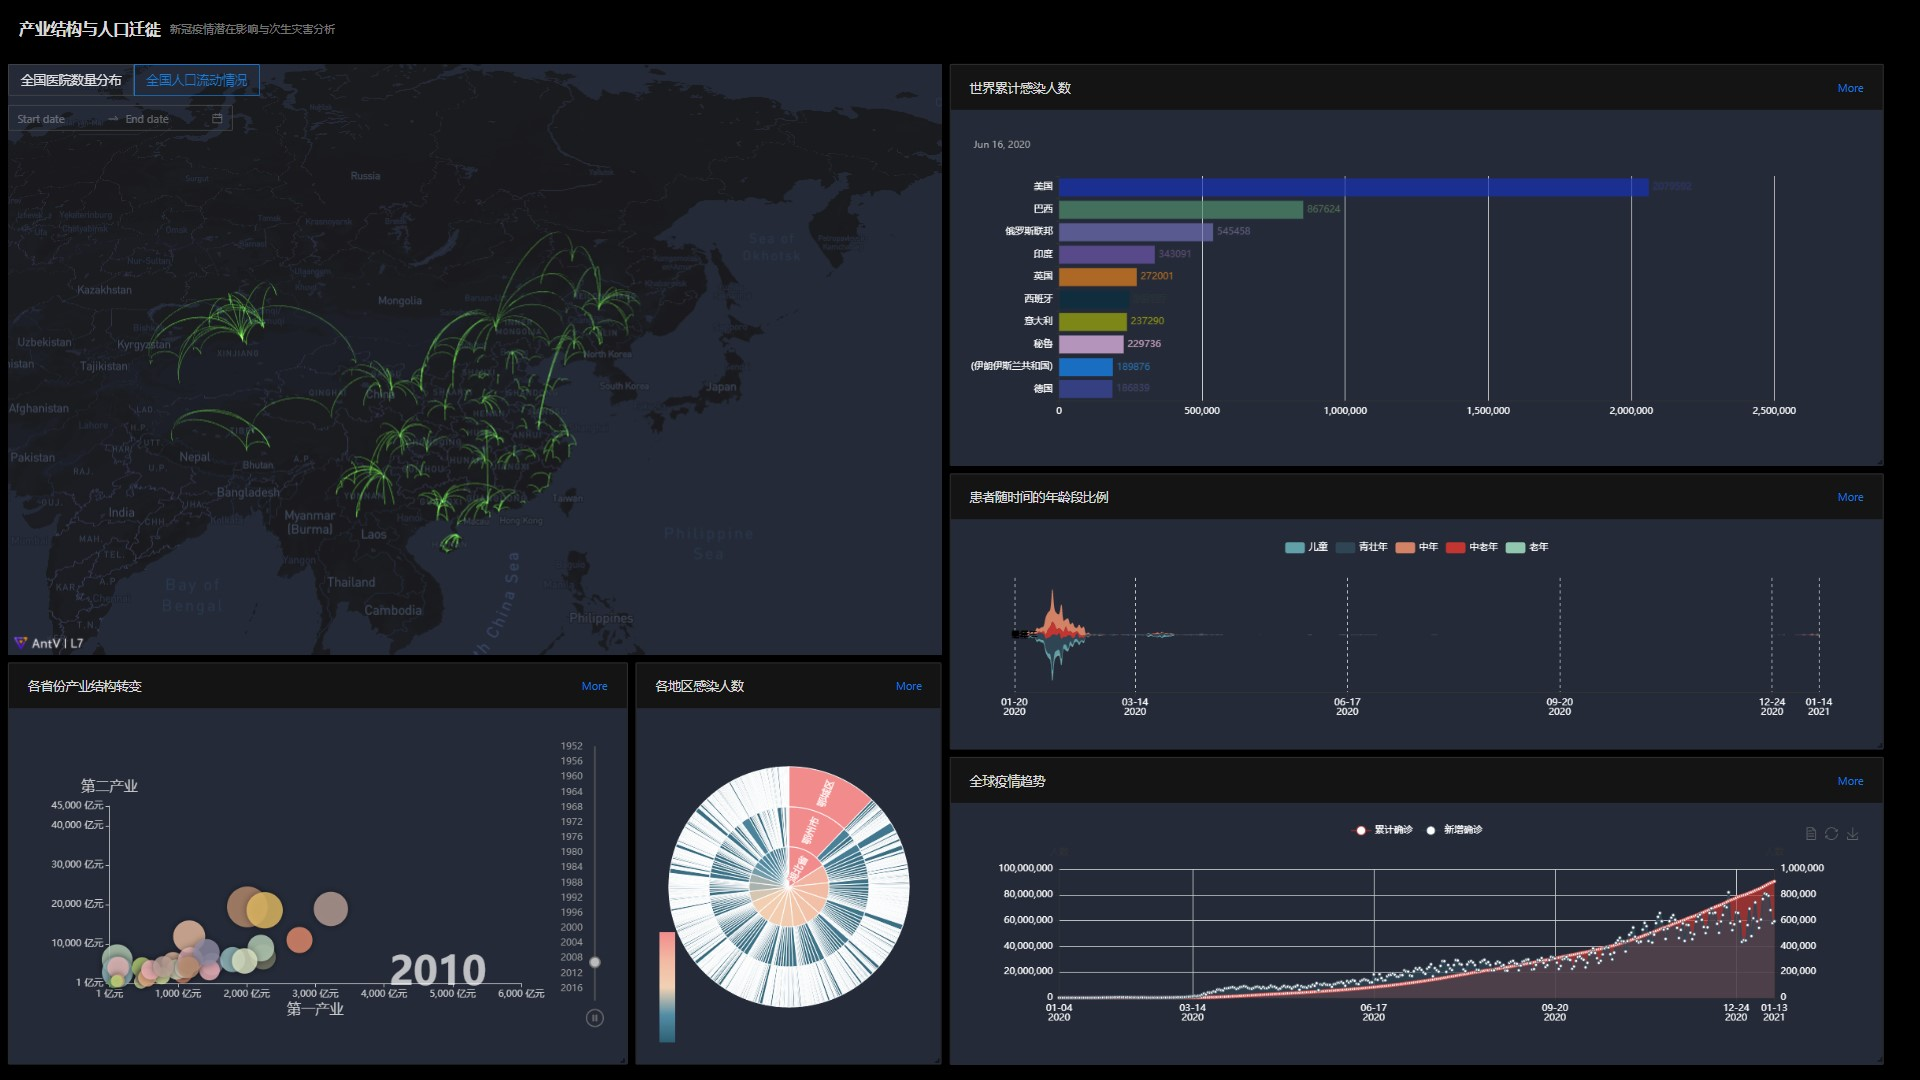
\includegraphics[width=0.9\textwidth]{img/panel}
    \caption{主面板界面}
    \label{}
\end{figure}
\begin{figure}[H]
    \centering
    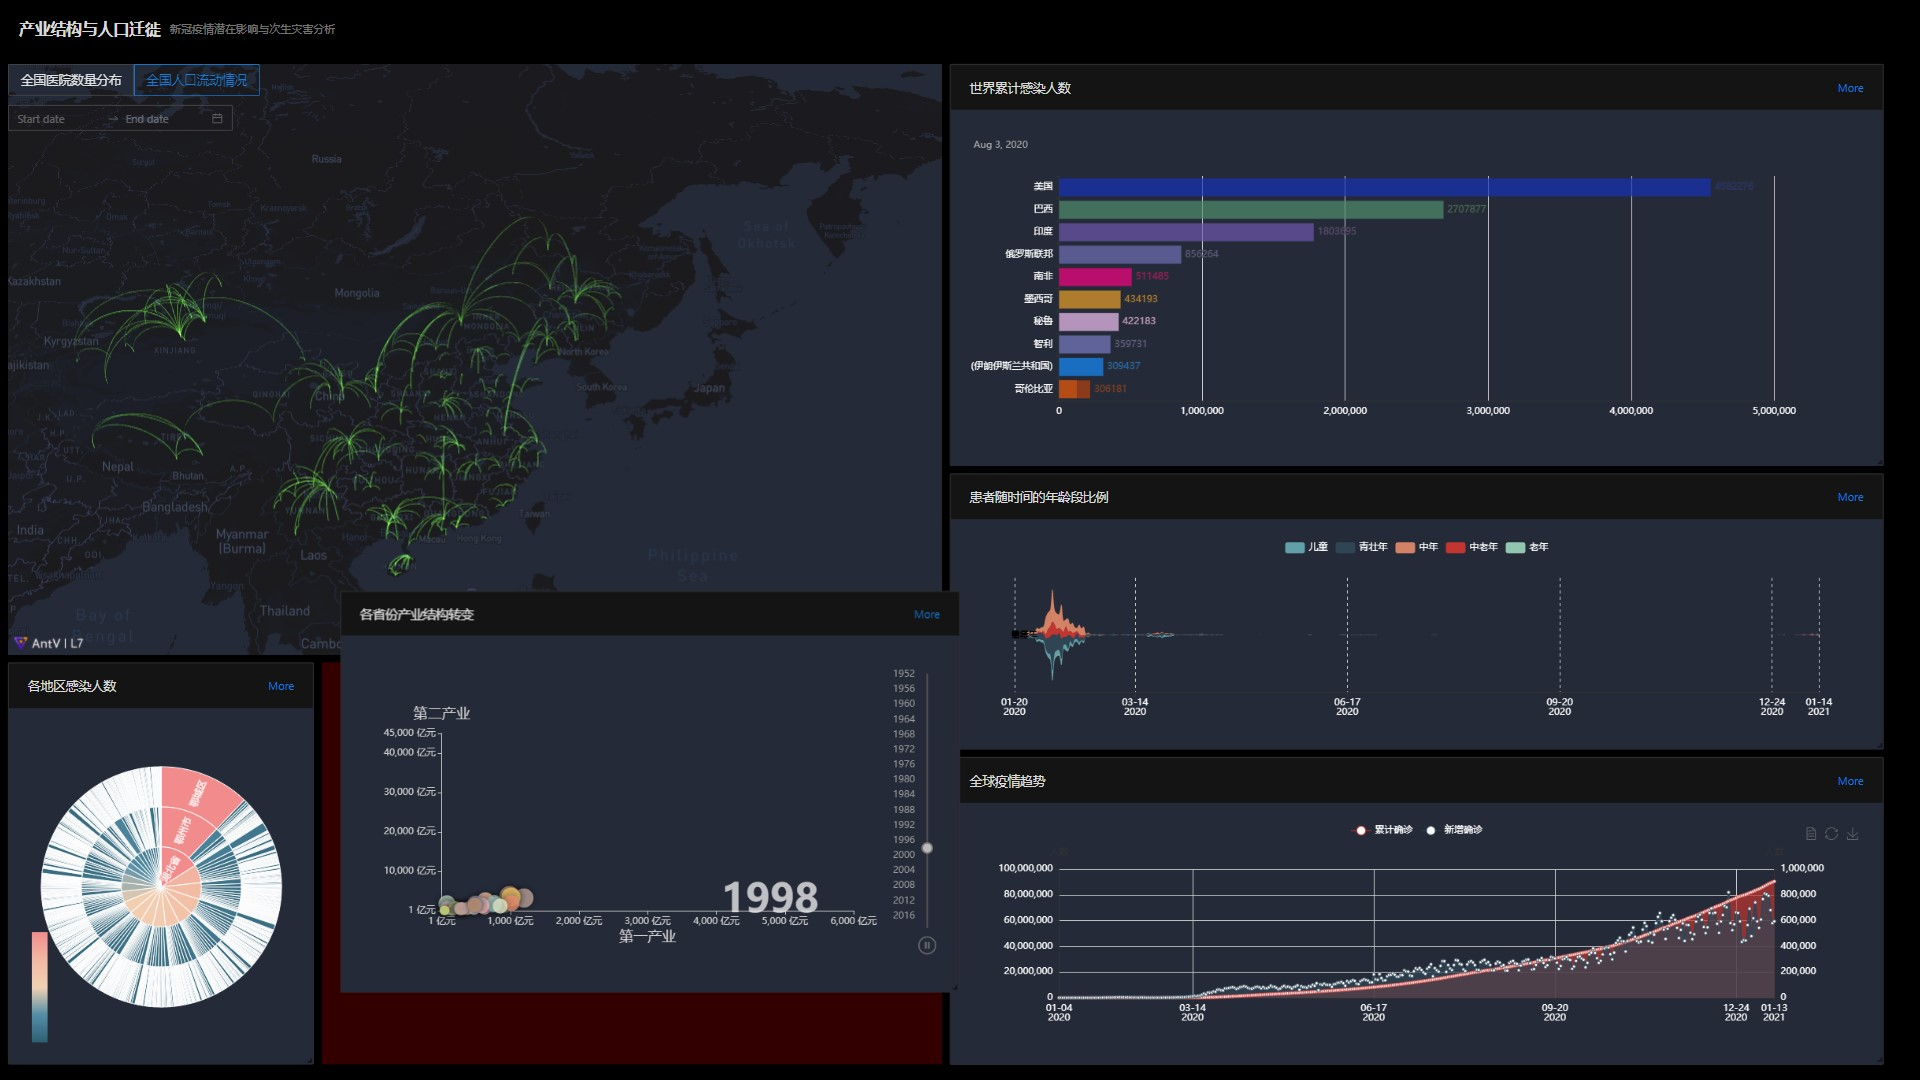
\includegraphics[width=0.9\textwidth]{img/paneldrag}
    \caption{主面板界面元素缩放}
    \label{}
\end{figure}
\newpage
\begin{figure}[H]
    \centering
    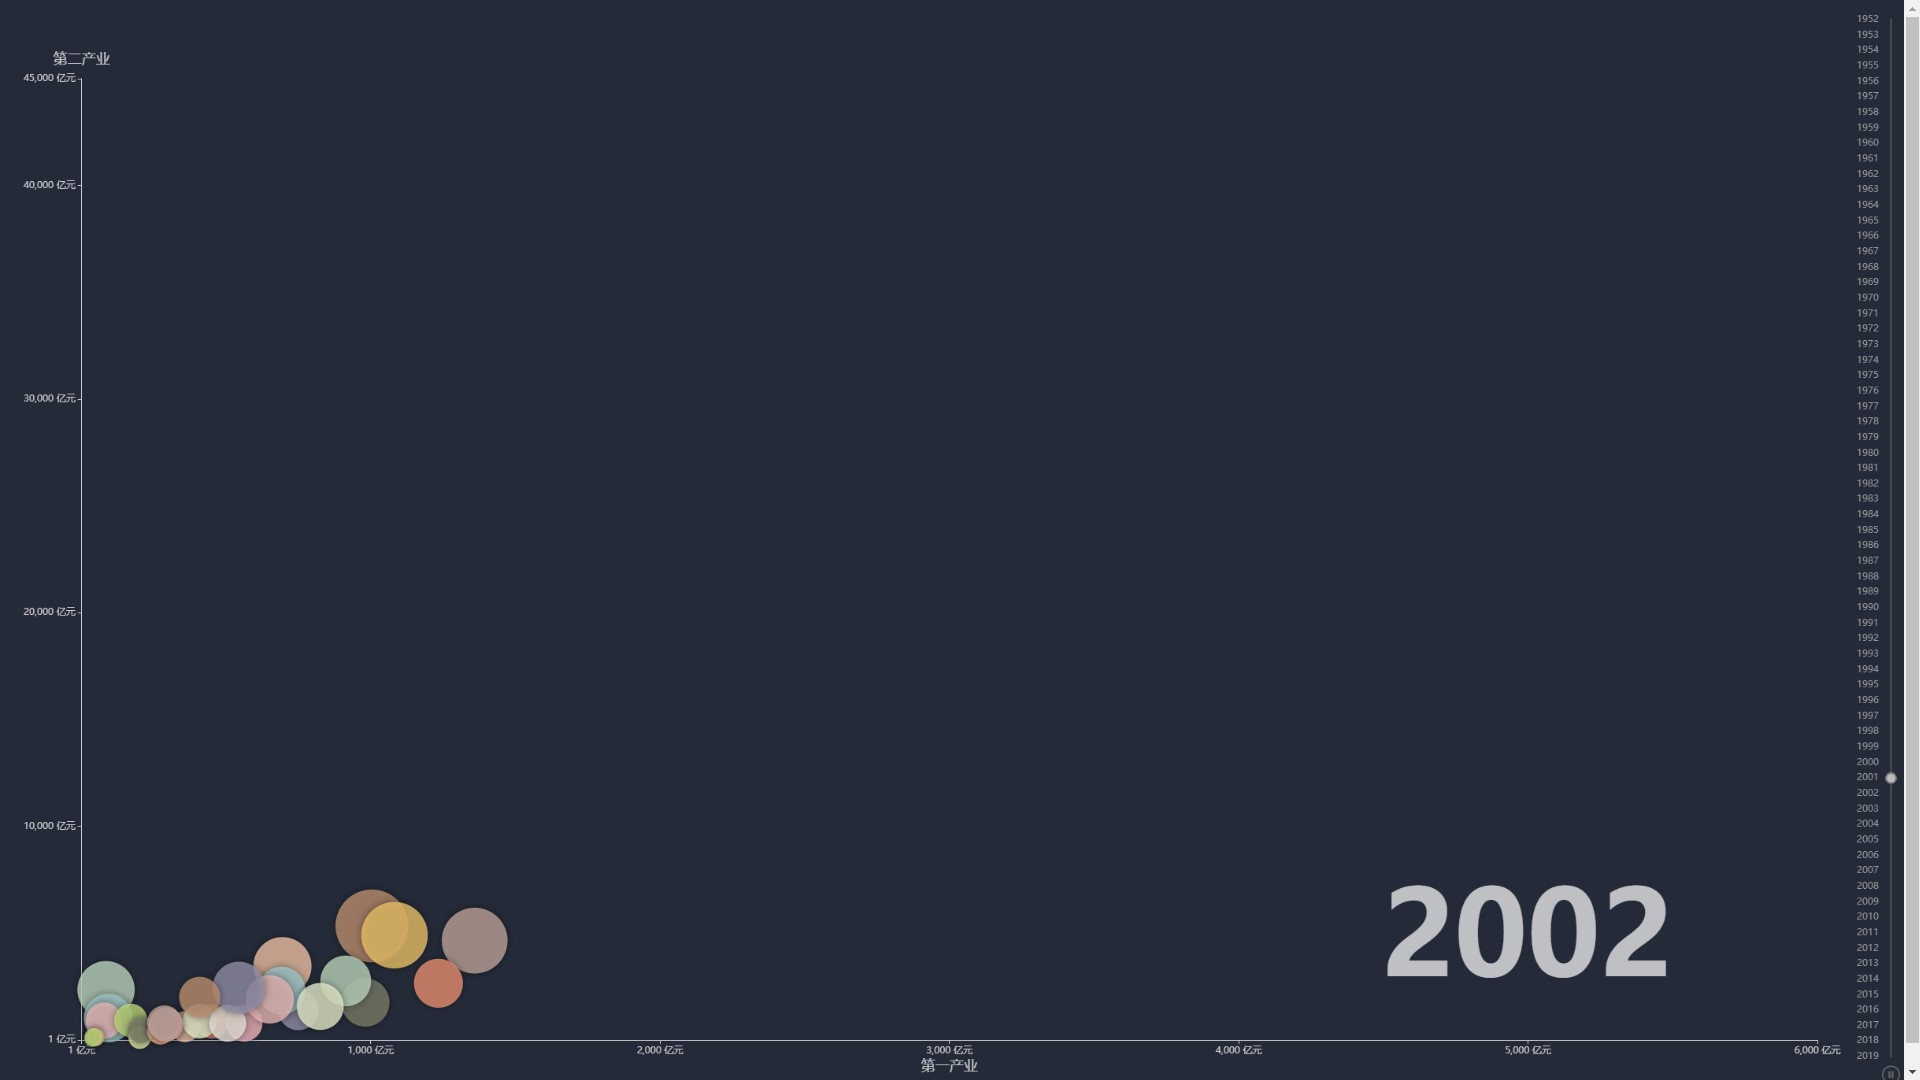
\includegraphics[width=0.9\textwidth]{img/panelmore}
    \caption{主面板界面元素放大到全屏}
    \label{}
\end{figure}
\newpage
\subsection{人口迁徙与医院数量分布}

\begin{figure}[H]
    \centering
    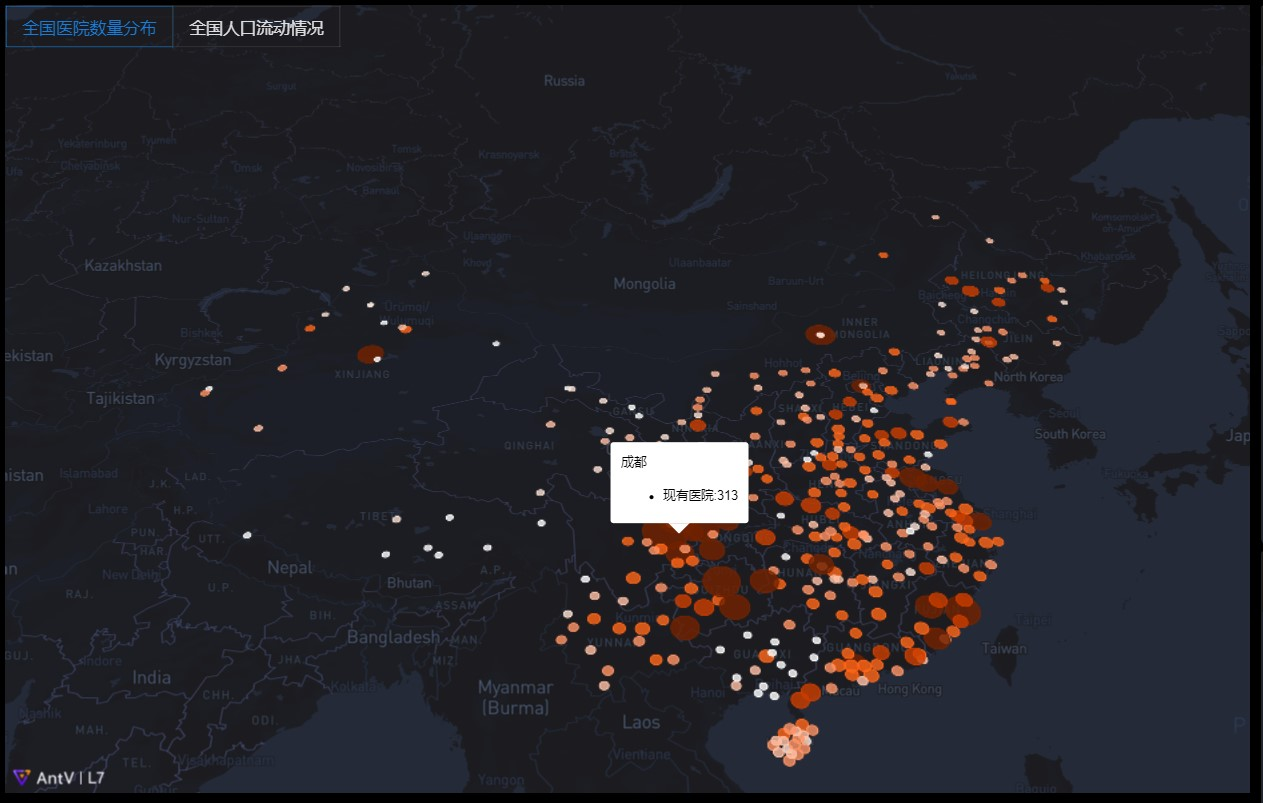
\includegraphics[width=0.9\textwidth]{img/hospitalNum}
    \caption{医院数量分布}
    \label{}
\end{figure}
\begin{figure}[H]
    \centering
    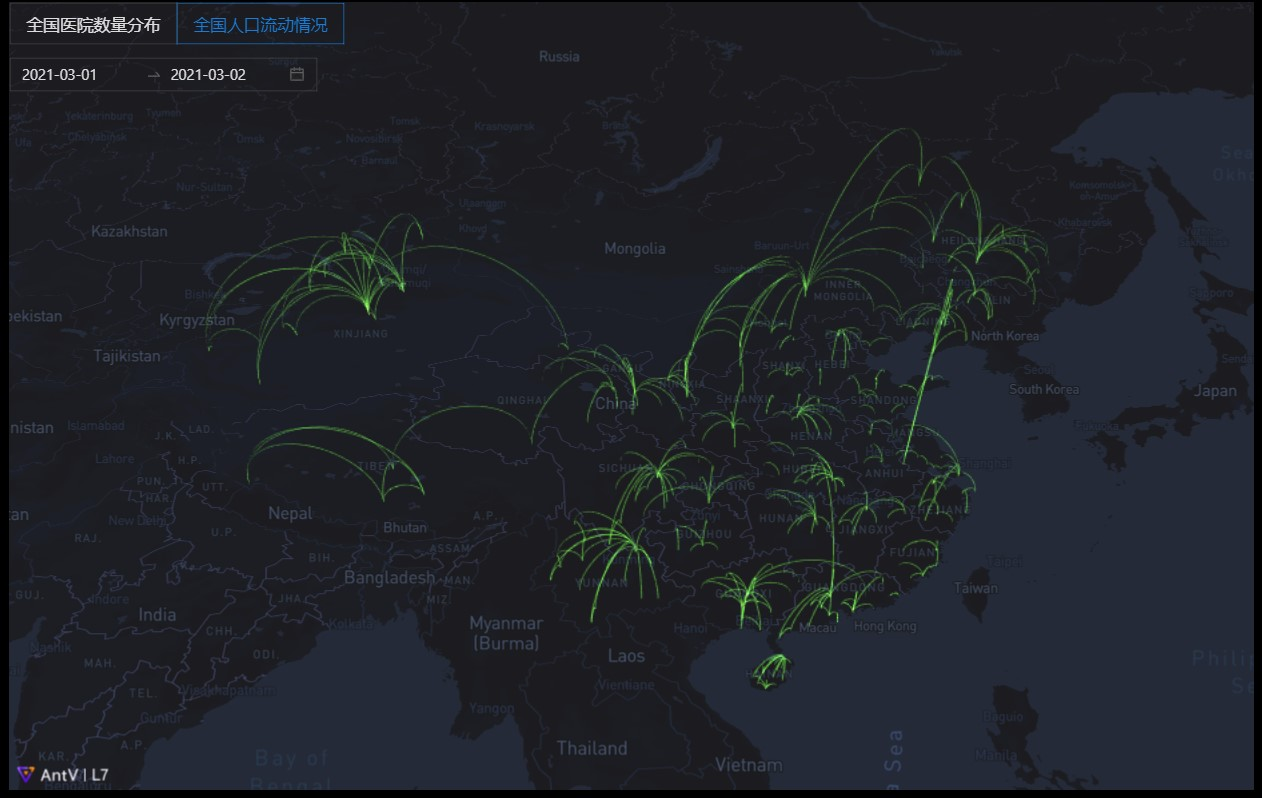
\includegraphics[width=0.9\textwidth]{img/gather}
    \caption{人口迁徙分布}
    \label{}
\end{figure}
我们可以看到,人口迁徙还是体现了区域的集聚性,并不是大规模大距离的迁徙,即便是春运期间。同时,迁移方向和医院的分布并没有显著的相关性。在切换迁徙时间的过程当中,我们可以看到,在春运期间区域积聚相对不明显,迁移较大,而其他时间积聚显著多于春运期间。可以看出,往东南沿海城市和往省会城市迁徙仍然是占据了比较大的迁移比重。
\subsection{患者随时间的年龄段比例}
\begin{figure}[H]
    \centering
    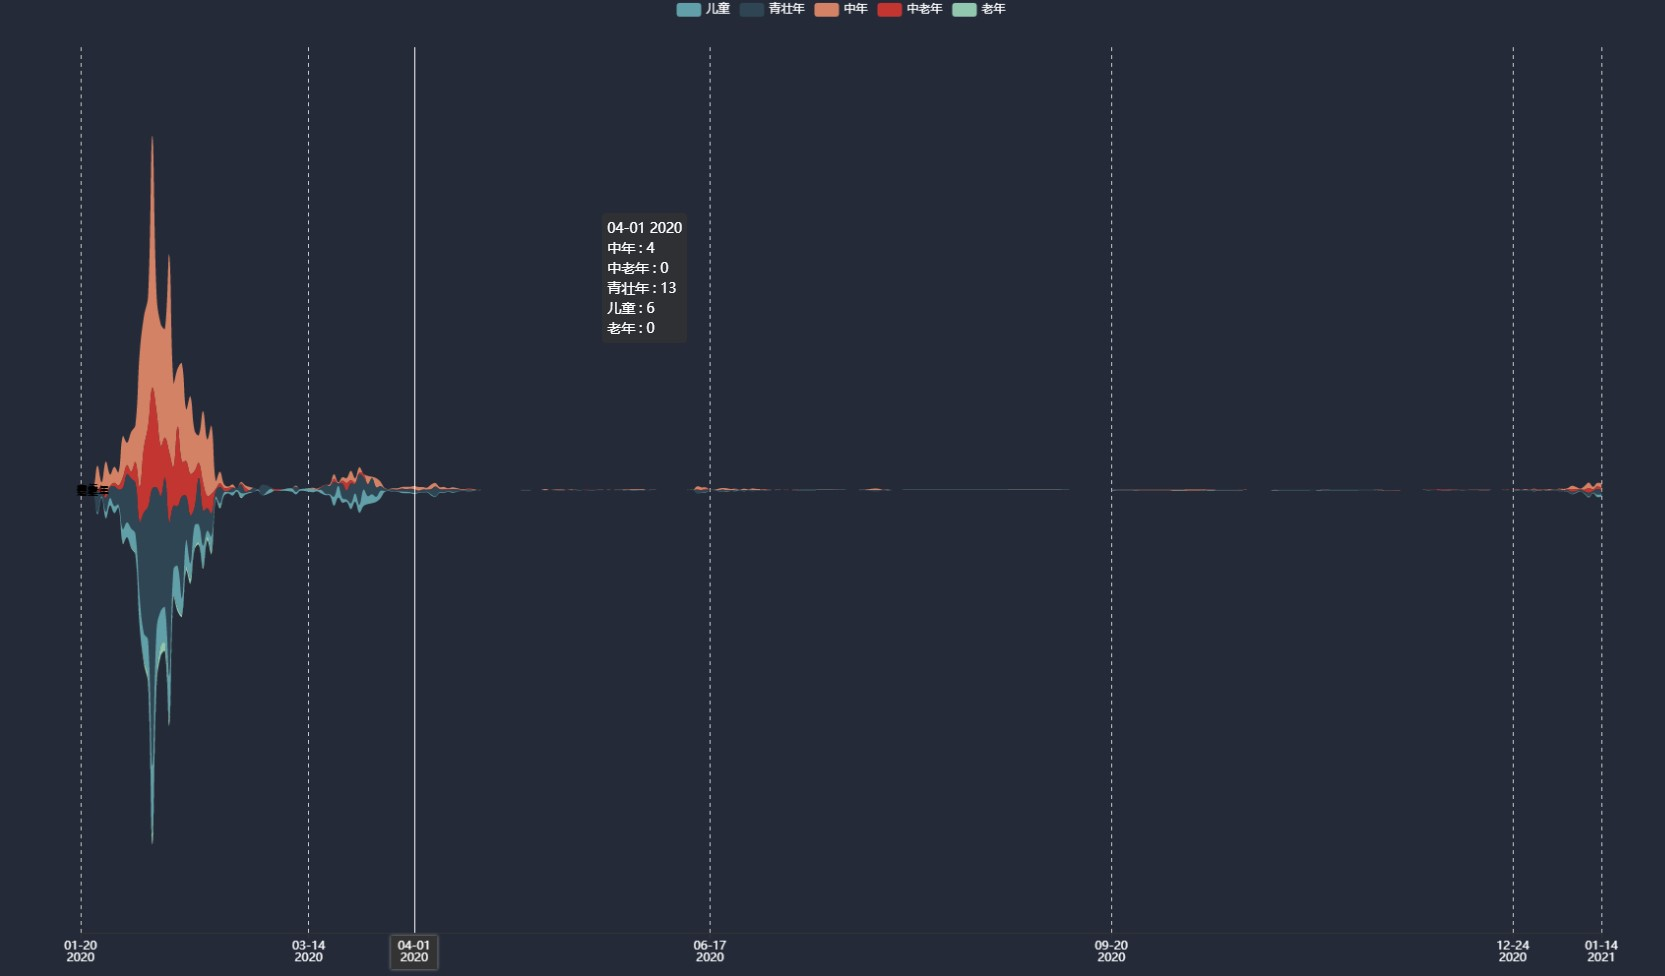
\includegraphics[width=0.9\textwidth]{img/age}
    \caption{患者随时间的年龄段比例分布}
    \label{}
\end{figure}
从数量上可以看出,我国的疫情在年初达到了一波高峰,但是很短暂,很快就控制了疫情。从不同颜色的河流可以看出,疫情的发展态势没有明显改变到不同年龄段受疫情的影响。同时,各个年龄段受疫情的影响也没有显著的差异。由此可以看出,各个年龄段都容易感染新冠肺炎,各个年龄段都应该注意好防护,万万不可掉以轻心。
\subsection{各省份产业结构变化趋势}
\begin{figure}[H]
    \centering
    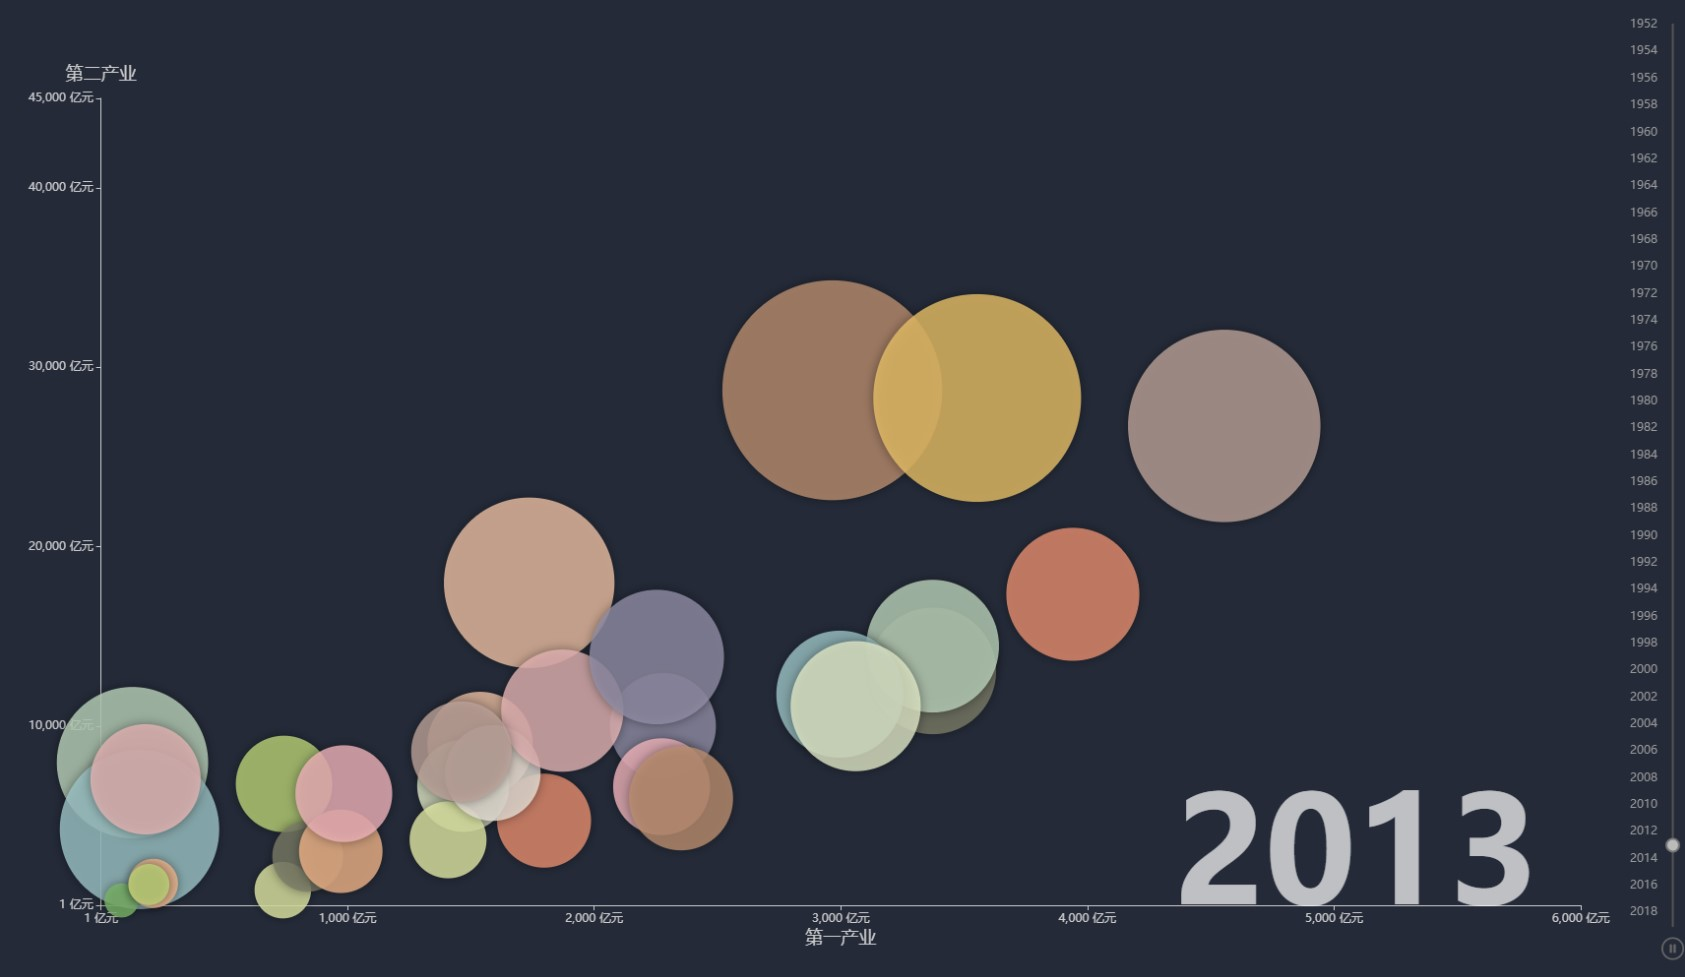
\includegraphics[width=0.9\textwidth]{img/GDP}
    \caption{各省份产业结构变化趋势}
    \label{}
\end{figure}
我们可以看到在经济发展的重要转型时期,例如改革开放,整个图的格局会发生比较大的变化。从2010到2020年几年间,各个省份位于坐标轴上的位置相对固定。可以预见的是,以第一产业第二产业为核心的省份,收到经济冲击较大,而以北京、上海等发达城市以第三产业为主,相对影响较小。同时,从客观的角度来讲,疫情加速了企业线上办公的进程,促进了产业的转型。由于2020年的完整GDP数据还没有公布,我们只能做一个初步预期,同时在统计局公布后(1/18)将数据集放进去可以和我们的猜想进行交叉验证。
\subsection{各个区域披露数据的比例}
\begin{figure}[H]
    \centering
    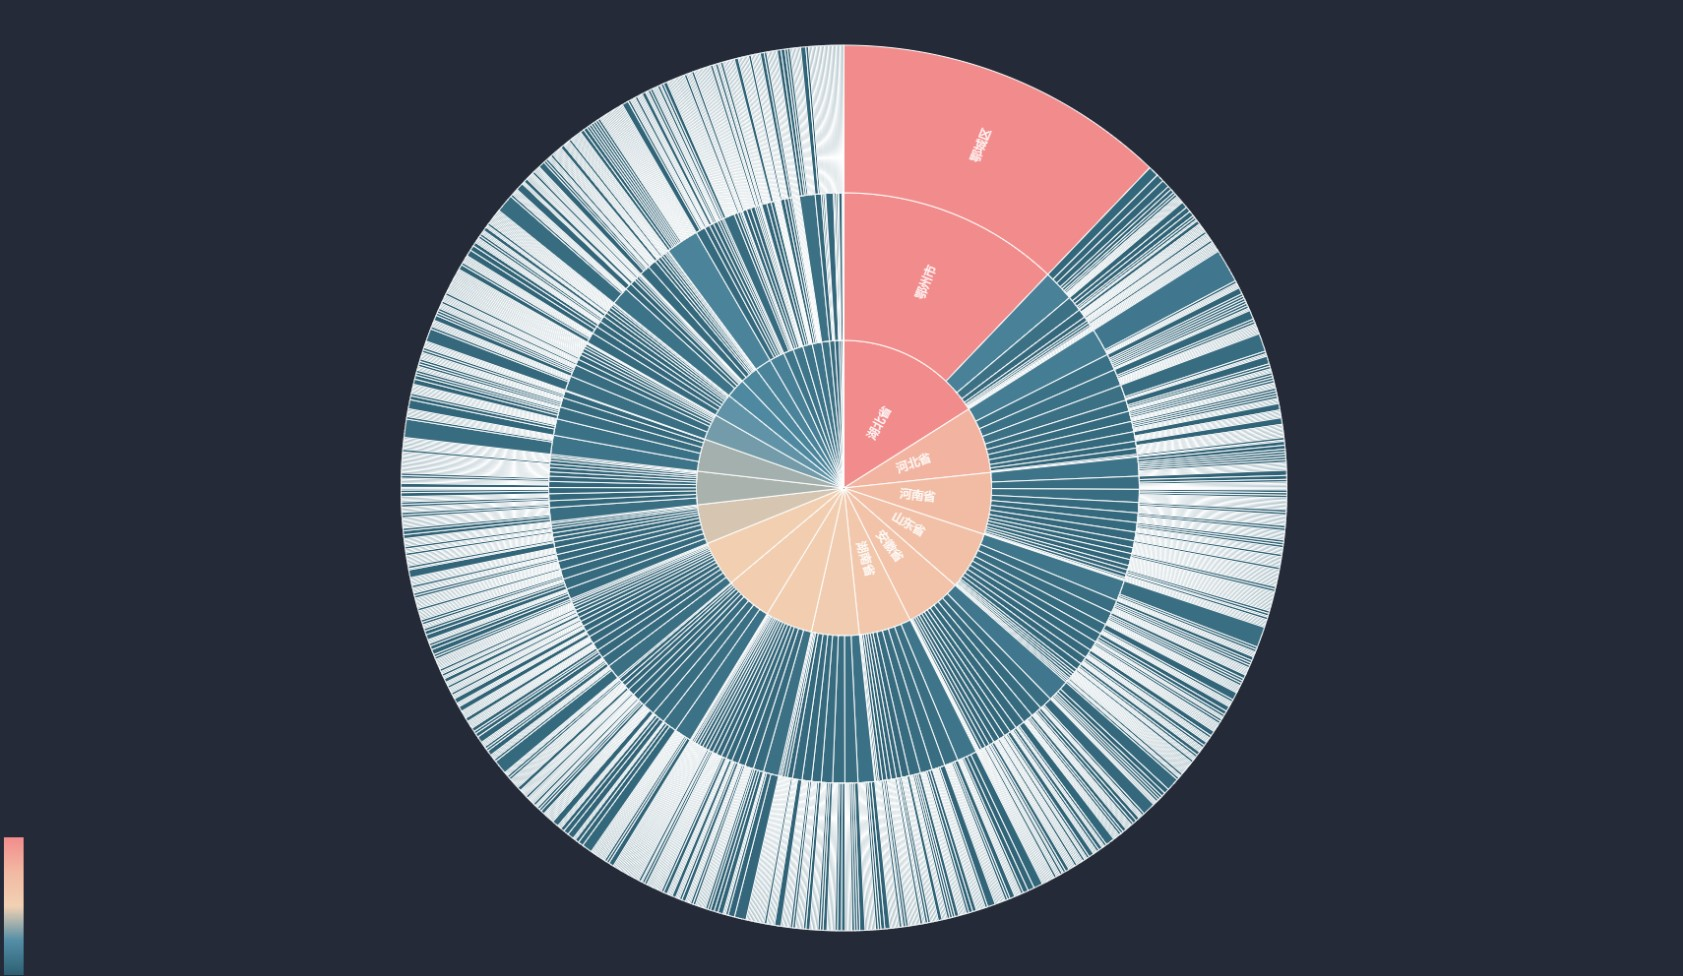
\includegraphics[width=0.9\textwidth]{img/sunburst}
    \caption{各省份产业结构变化趋势}
    \label{}
\end{figure}
借助颜色和形状的视觉通道,我们可以看到各个省份的披露患者数据的比例,为了更好地应对疫情的蔓延趋势,各个省份对于每一位病患所在区域进行严格把控。然而,疫情初期,很多对于疫情的追踪并不到位。从图中可以看出,尽快湖北是中国疫情最为严重的区域,但是其披露的数据仅仅只有全部披露数据的四分之一。这也印证了疫情初期的披露数据还有提升的空间。
\subsection{世界疫情发展趋势}
\begin{figure}[H]
    \centering
    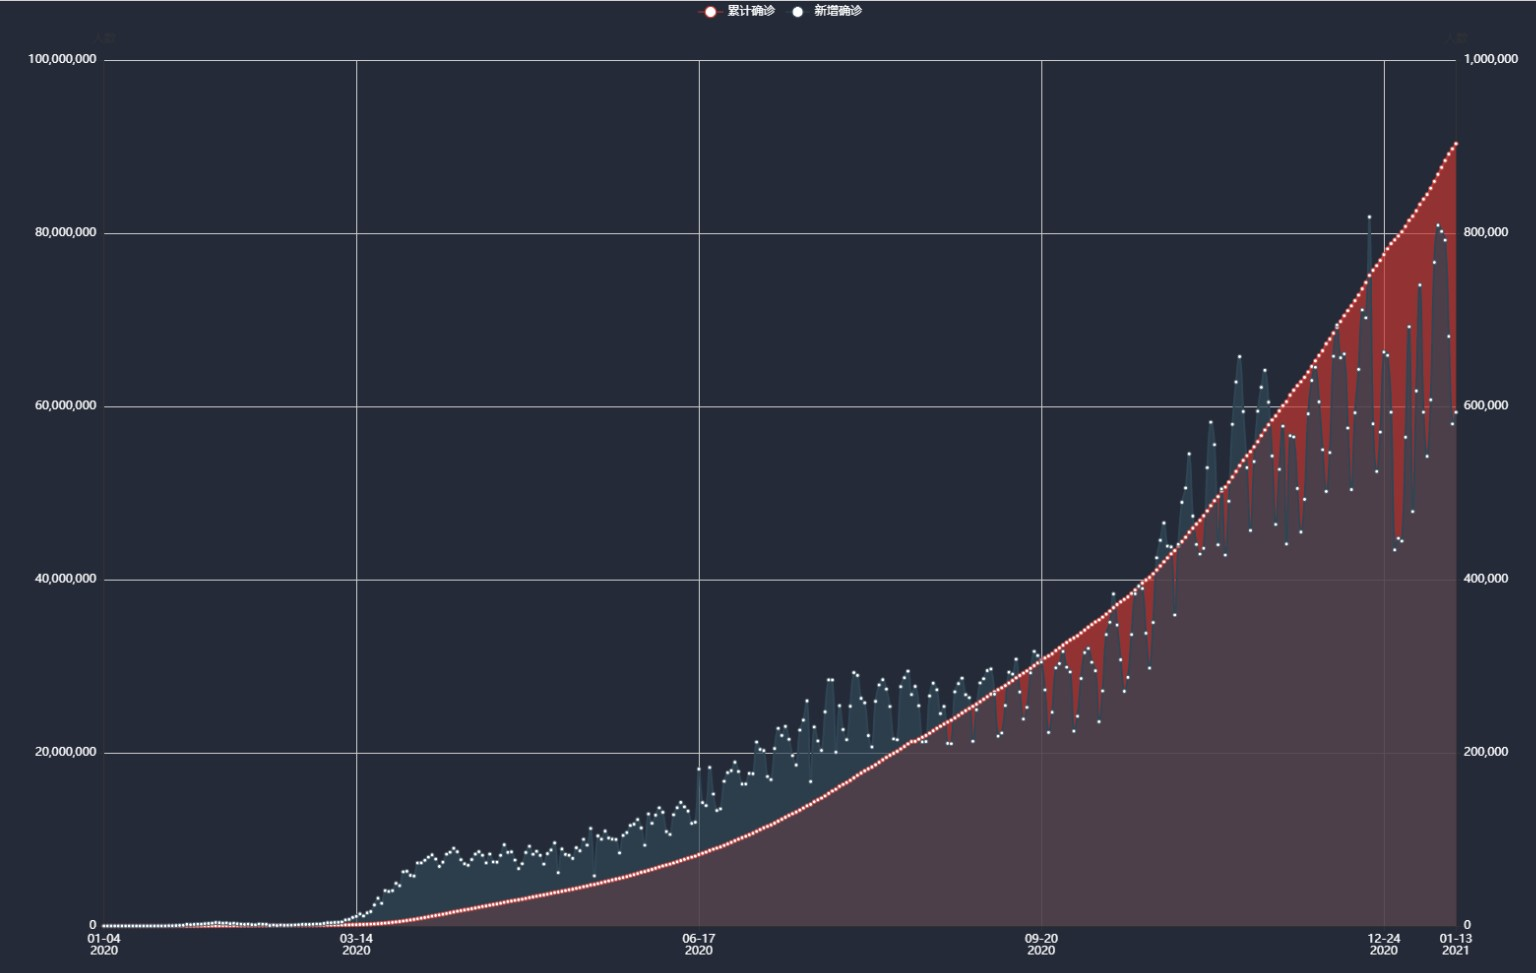
\includegraphics[width=0.9\textwidth]{img/worldtrend}
    \caption{世界疫情发展趋势}
    \label{}
\end{figure}
从图中可以看出,世界的疫情发展态势截止到目前为止依然是不容乐观,确诊人数长期处于上升状态。可以预计,在未来很长一段时间里,疫情都将是一个常态,成为生活当中尤其是有国外交流需求的生活当中的一个重要组成部分。同时,在经济上,也将持续影响着我们的生活,带来经济下行压力和客观上促进经济转型。
\subsection{疫情最严重的国家排名}
\begin{figure}[H]
    \centering
    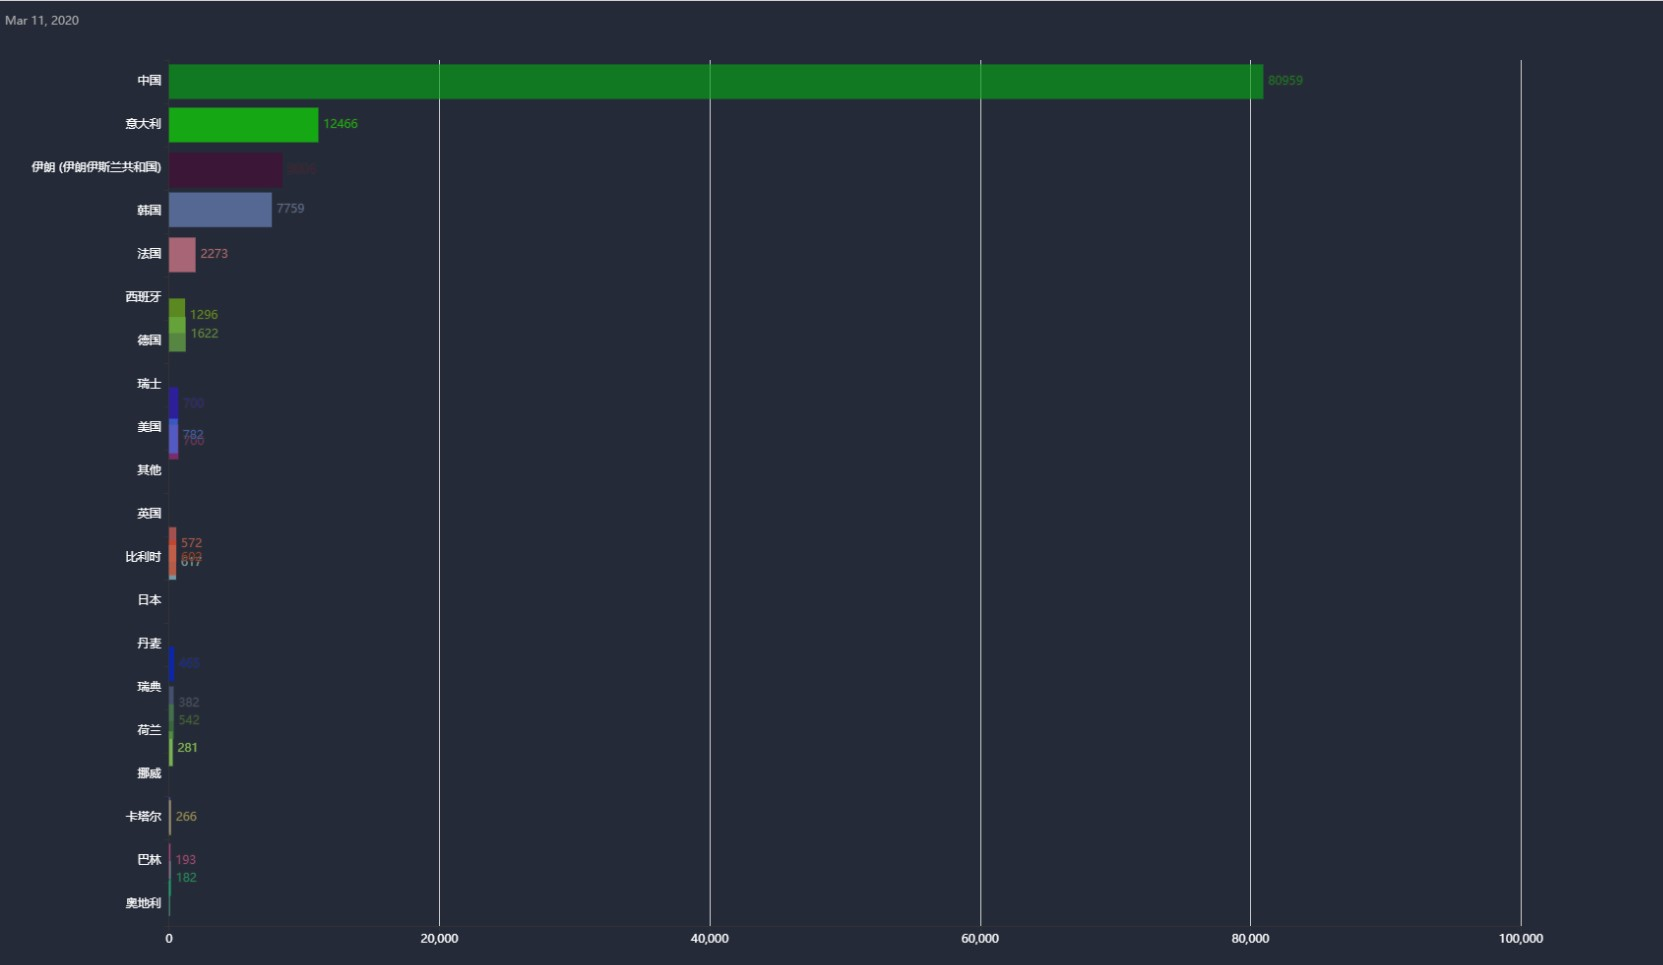
\includegraphics[width=0.9\textwidth]{img/begin}
    \caption{2020年3月份各国疫情状态}
    \label{}
\end{figure}
\begin{figure}[H]
    \centering
    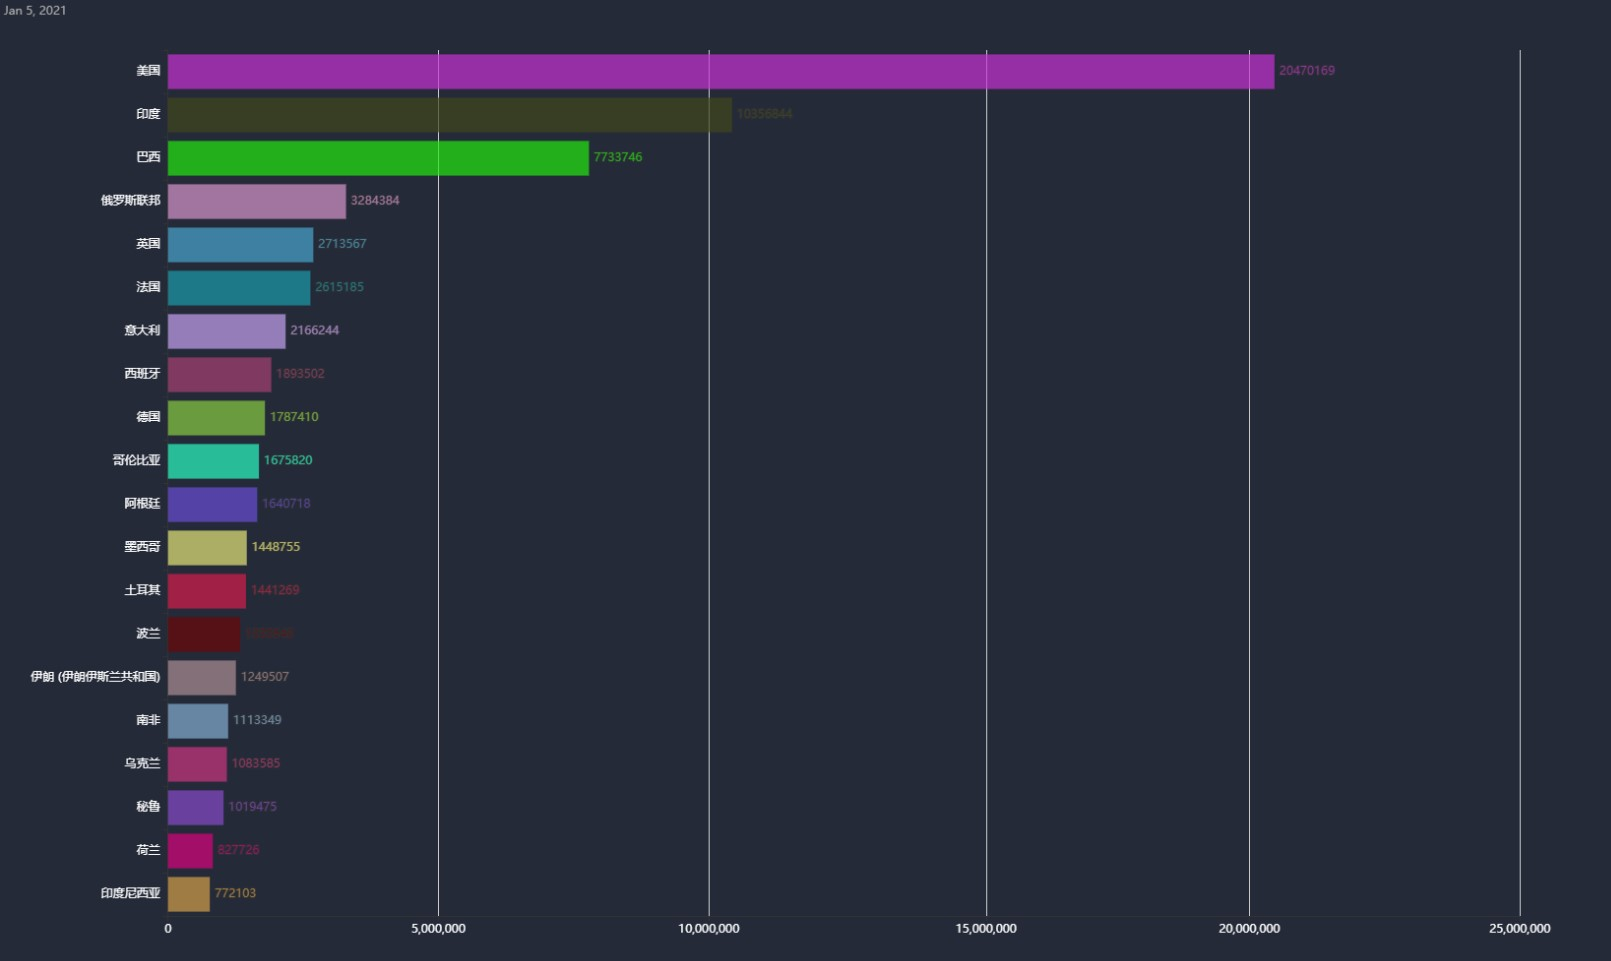
\includegraphics[width=0.9\textwidth]{img/end}
    \caption{2021年1月份各国疫情状态}
    \label{}
\end{figure}
从变化的数据可以看出,尽管中国在早期是疫情最为严重的国家,但是很快就控制住了疫情。然而以美国为首的很多西方国家对于疫情没有足够的危机意识,即便在有中国的先例之后依然没有很好地控制住疫情,严重拖累了世界范围内疫情的诊断治疗,并且持续了非常长的一段时间,直至今天。疫情国家的排名变化非常具有对比和冲击力,尤其是中国慢慢推出排行榜的过程和美国不断霸榜并远超第二名。
\end{document}